\documentclass{article}

% packages
\usepackage[english]{babel}
\usepackage[utf8]{inputenc}
\usepackage{amsmath}
%\usepackage{amssymb}
%\usepackage{amsthm}
\usepackage{braket}
\usepackage{graphicx}
%\usepackage{bbm}
%\usepackage{multirow}
\usepackage{tikz}
\usetikzlibrary{positioning}
\usetikzlibrary{shapes.arrows}
\usepackage{color}
%\usepackage[colorinlistoftodos]{todonotes}
%\usepackage[absolute,overlay]{textpos}
%\usepackage{hyperref} % Should be last package imported
\usepackage{fullpage}

%%%%%%%%%%%%%%%%%%%%%%%%%%%%%%%%%%%%%%%%%%%%%%%%%
%%% SHORTCUTS %%%

%\newcommand{\pagehline}{\\\specialrule{.01pt}{0pt}{5pt}}
\newcommand{\pagehline}{\noindent\rule{\textwidth}{0.2pt}}

\newcommand{\paren}[1]{\left( #1 \right)}
\newcommand{\expectation}[1]{\left< #1 \right>}
\newcommand{\brac}[1]{\left[ #1 \right]}
\newcommand{\zerodel}{.\kern-\nulldelimiterspace}
\newcommand{\abs}[1]{\left\vert #1 \right\vert}
\newcommand{\wt}[1]{\widetilde{#1}}

\newcommand{\vecE}{\mathbf{E}}
\newcommand{\vecB}{\mathbf{B}}
\newcommand{\kvec}{\mathbf{k}}
\newcommand{\xvec}{\mathbf{x}}
\newcommand{\rvec}{\mathbf{r}}
\newcommand{\bvec}{\mathbf{b}}
\newcommand{\Rvec}{\mathbf{R}}
\newcommand{\zbar}{\overline{z}}
\newcommand{\curl}{\nabla\times}
\renewcommand{\div}{\nabla\cdot}

\DeclareMathOperator{\Lagr}{\mathcal{L}}
\DeclareMathOperator{\Ham}{\mathcal{H}}
\DeclareMathOperator{\tr}{tr}

\newcommand{\lucas}[1]{\textcolor{blue}{\bf [LKW #1]}} % Lucas comment


\begin{document}

\begin{center}
{\Large Fitting a band structure model for silicon}
\end{center}

\section{Mean field calculation}

A conventional silicon cell was used (diamond structure) with 8 Si atoms (16 up electrons, 16 down).
Kohn-Sham orbitals were computed at the gamma point using DFT.
DFT was run in PySCF using the PBE xc-functional and BFD pseudopotentials.
There are 16 occupied orbitals in the lowest energy mean-field wave function.


\section {Two states: exciting one electron}

\noindent {\bf Selecting determinants and wave function samples}

The first goal is a simple calculation that can improve the energy estimate of a single particle excitation.
From the mean-field (DFT) states, two determinants are selected: the lowest energy determinant $S_0$, and the next determinant $S_1$, promoting one up electron from the highest occupied to lowest unoccupied state.
Ten sample states are generated by choosing different weights for these two determinants,

\[ \Psi_i^S = c_{i0}S_0 + c_{i1}S_1 \]

where $c_{i1}/c_{i0}$  is varied from 0 to 1.8.

A Jastrow factor is optimized for each two-determinant function $\Psi_i^S$,

\[\Psi_i = \Psi_i^S \Psi_i^J,\]

and the one-body density matrices are computed by VMC.


\begin{figure}[h]
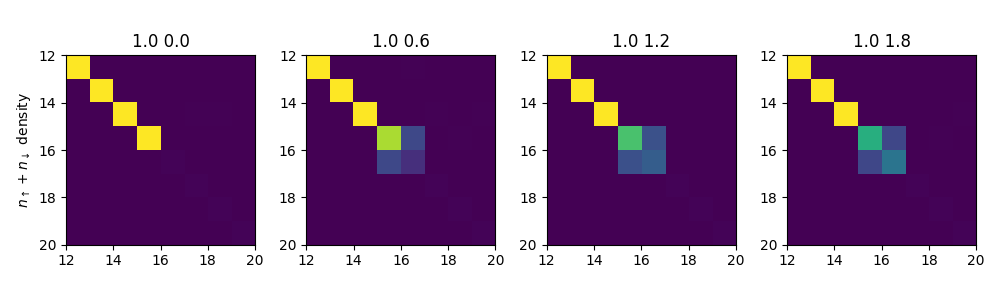
\includegraphics[width=0.5\textwidth]{images/vmc_obdm.png}
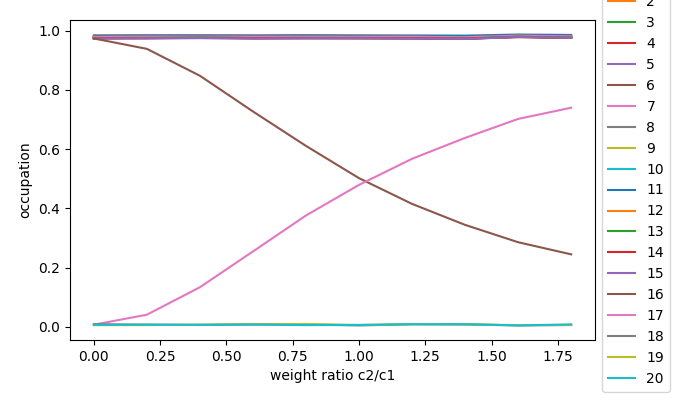
\includegraphics[width=0.5\textwidth]{images/vmc_occupations.png}
\caption{
(Left) Part of the one-body density matrix computed from different wave functions, showing the matrix elements that change across samples. 
(Right) The orbital occupations (diagonal of OBDM) plotted against determinant weight $c_1$.
}
\label{fig:obdm}
\end{figure}

\noindent {\bf Descriptors }

Only the occupations of orbitals 16 and 17 change noticeably across samples.
The two determinants have either orbital 16 or 17 occupied, and all other occupations are the same, so this is not surprising, and the population of orbital 17 increases with the weight of determinant $S_1$.
This tells us only orbitals 16 and 17 can be relevant to the model.
Since the trace of the OBDM is the number of electrons ($n_{16}+n_{17}=2$), there is only one free parameter, which I choose to be $n_{17}$.

\noindent {\bf Fitting a model }

The model is 
\[
\expectation{H} = E_0 + \epsilon_1 \expectation{\hat{n}_{17}};
\]

there is a constant energy shift $E_0$ and a term proportional to $n_{17}$, the occupation of orbital 17, with coefficient $\epsilon_{1}$, which should be the energy of the one-particle excitation.
Using least squares regression, I computed $E_0$ and $\epsilon_1$, and compare the fit to the data points from VMC.

\begin{figure}
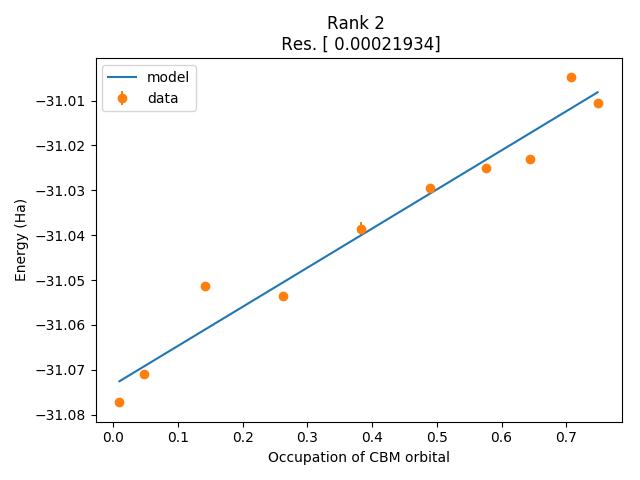
\includegraphics[width=0.5\textwidth]{images/vmc_2orb_model.png}
\caption{
Energy vs occupation $n_{17}$. The line is the linear fit, the points are from simulation (with error bars in both energy and density).
}
\label{fig:model}
\end{figure}




\end{document}
